





\section{Softmax Collapse: Floating Point Errors Prevent Grokking} \label{sec:floating_points}

Given our current understanding of grokking, it is surprising that it happens without regularization for some dataset sizes, but regularization becomes crucial as dataset size decreases \citep{power2022grokking}. In this section we highlight that looking at datasets at the boundary of these two regimes reveals that without weight decay, grokking sometimes starts before abruptly stopping (\cref{fig:grokking_stops}). We show that this is caused by floating point errors in the \softmax that lead the gradients from a large fraction of the samples to become zero. We refer to this phenomenon as Softmax Collapse. 

\subsection{Softmax Collapse}

In modern neural network implementations, Floating Point (FP) arithmetic is ubiquitous for representing and computing parameters, activations, and gradients. While FP numbers enable efficient decimal computations, they introduce numerical inaccuracies. This section focuses on \textit{absorption errors}, as a specific class of FP arithmetic failure. We will use the symbol $\doteq$ to refer to equality under FP arithmetic.

\begin{dfn}[Absorption Errors]
Let $a, b \in \mathbb{R}\setminus\{0\}$ be floating point numbers in a system with base $\beta$ and $p$ significand bits. Denote their exponents by $e_a$ and $e_b$, respectively. An \emph{absorption error} occurs in the computation of $a + b$ (denoted $a + b \doteq a$) if
\[
e_a - e_b \geq p.
\]
In this case, after exponent alignment, the significand of $b$ is shifted right by at least $p$ digits, and $b$ cannot be represented in the available precision, resulting in $a + b \doteq a$.
\end{dfn}

Intuitively, absorption errors can occur during FP addition when operands have significantly different magnitudes. For $float32$ the base $\beta$ is 2 and $p=24$ bits, meaning that adding any number smaller than $2^{-(p-1)}=2^{-23} $ to 1 will leave 1 unchanged. $2^{-23}$ is the machine epsilon for float32.

\paragraph{Absorption errors in the $\bfsoftmax$}
The $\softmax$ function is a fundamental component in numerous deep learning architectures, serving as an activation function or a key element in attention mechanisms. In this case, we focus on its application within the Softmax Cross-Entropy (SCE) loss:

\begin{dfn}[Softmax Cross-Entropy (SCE) loss]
    For a neural network $f$ and a data point $\textbf{x}$ with label $y$, we define $\textbf{z} \coloneq f(\textbf{x})$ and $z_y$ as the logit corresponding to the true class $y$ . We express the SCE loss as well as its equivalent numerically more stable formulation as:
\begin{equation}
    \loss_{\mathrm{SCE}}(f(\textbf{x}), y) = -\log\left(\frac{e^{z_y}}{\sum_{k=1}^n e^{z_k}}\right)= -z_y + \max(\textbf{z}) + \log\left(\sum_{k=1}^n e^{z_k-\max(\textbf{z})}\right)
    \label{eq:log_softmax}
\end{equation}
\end{dfn}

Unfortunately, even the rightmost (comparatively more stable) variant does not address this problem, since the kind of FP errors discussed in this work appear in the sum. While the \softmax function outputs are bounded between 0 and 1, the intermediate calculations involve summing exponentials of both positive and negative logits. These values can span several orders of magnitude, particularly in scenarios with large logits where the loss approaches zero. This wide range of values creates conditions that lead to absorption errors -- leading to the phenomenon we call \textit{Softmax Collapse}.

\begin{dfn}[Softmax Collapse (SC)]
    A specific case of absorption error occurs when, for a given sample $\textbf{x}$, the logit from the correct class $z_y$ is significantly larger than the logits for all other classes. This floating-point absorption of smaller terms, which we call \textbf{Softmax Collapse}, occurs when:
    \begin{equation}
    \sum_{k=1}^n e^{z_k} \doteq e^{z_y} ~ ,
    \label{eq:softmax_collapse}
    \end{equation}
    in which case the SCE loss becomes:
    \begin{equation}
        \loss_{\mathrm{SCE}}(f(\textbf{x}), y) \doteq -\log\left(\frac{e^{z_y}}{e^{z_y}}\right) = 0 ~ .
    \end{equation}
\end{dfn} 

Thus, during SC the loss becomes identical to zero. Furthermore, for the correct class, the gradients become zero as well: 
%
\begin{equation}
    \frac{\partial{ \loss_{SCE}}}{\partial z_{c}} =  \frac{e^{z_c}}{\sum_{k=1}^n e^{z_k}}-\mathbb{1}_{\{c = y\}} \doteq 1 - \mathbb{1}_{\{c = y\}} ~ .
    \label{eq:derivative}
\end{equation}
%
While weights that contribute to the wrong classes can still get negative updates, we show that disappearance of the gradients from the correct classes is enough to inhibit grokking (\cref{fig:grokking_stops}). We validate this in \cref{app:sc_intervention} with an explicit intervention, showing that artificially setting the gradients from the correct class to zero stops generalization in a very similar way to what we observe in \cref{fig:grokking_stops}.


\subsection{Evidence of Softmax Collapse in grokking tasks}

\begin{figure}[t]
\centering
\begin{subfigure}{.32\textwidth}
  \centering
  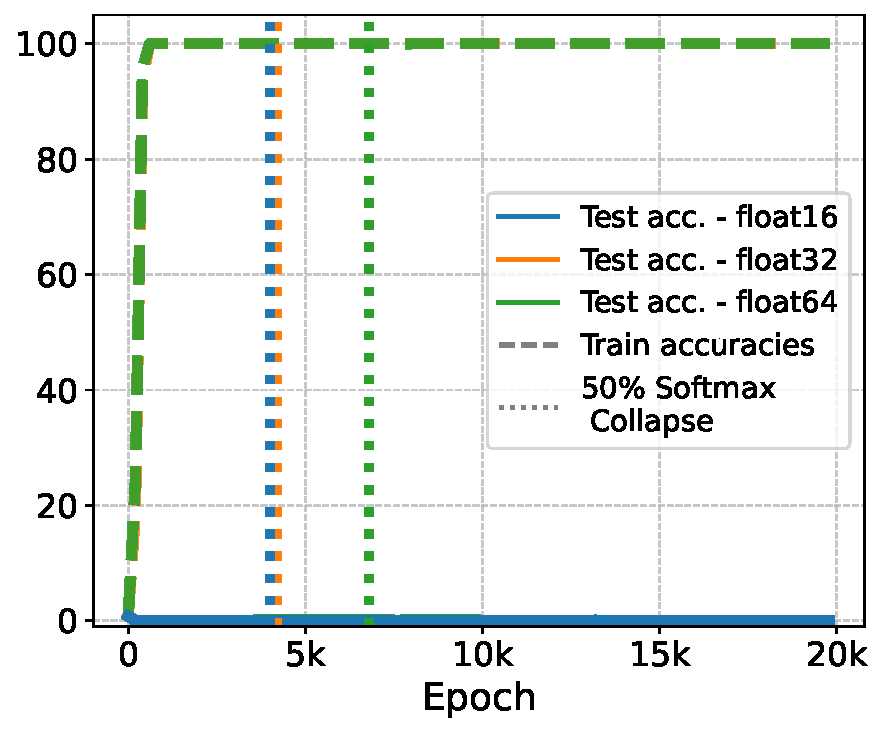
\includegraphics[width=\linewidth]{grokking_iclr_arxiv/figures/float32vsfloat64_40_percent_with_legend.pdf}
  \caption{40\% training data}
  \label{fig:grokking_stops_40}
\end{subfigure}
\hfill
\begin{subfigure}{.32\textwidth}
  \centering
  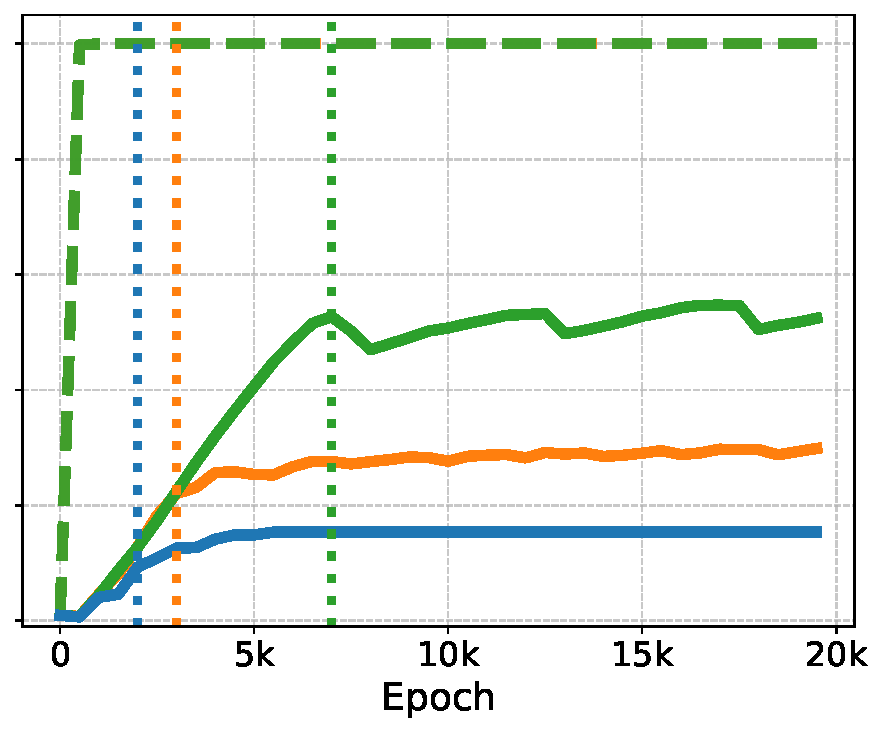
\includegraphics[width=\linewidth]{grokking_iclr_arxiv/figures/float32vsfloat64_60_percent.pdf}
  \caption{60\% training data}
  \label{fig:grokking_stops_60}
\end{subfigure}
\hfill
\begin{subfigure}{.32\textwidth}
  \centering
  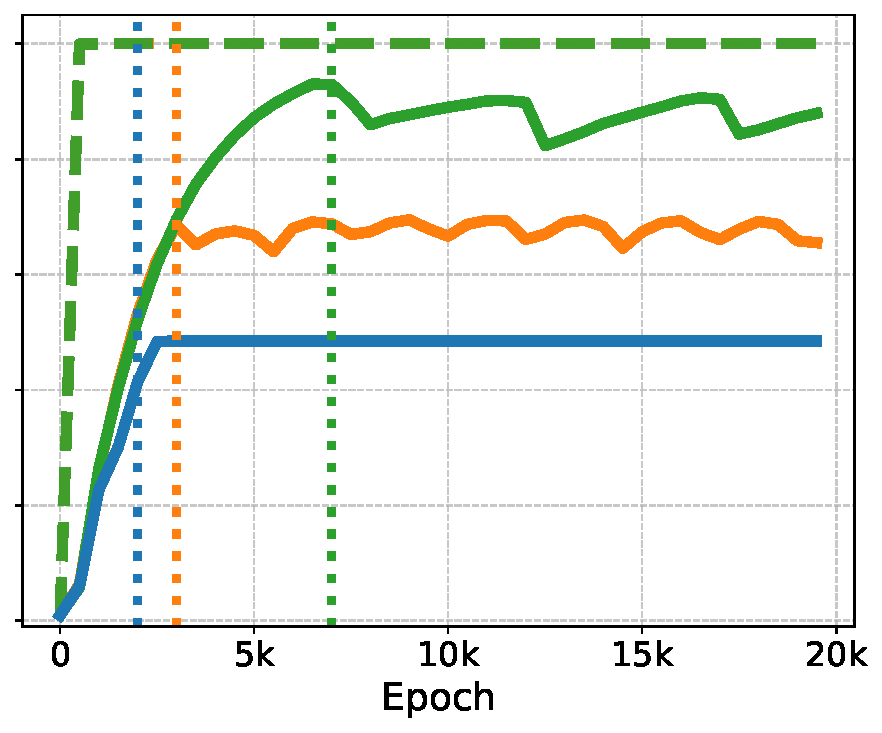
\includegraphics[width=\linewidth]{grokking_iclr_arxiv/figures/float32vsfloat64_70_percent_no_legend.pdf}
  \caption{70\% training data}
  \label{fig:grokking_stops_70}
\end{subfigure}
% \vspace{-3mm}
\caption{As dataset size increases (subplots \textbf{a} to \textbf{c}), MLPs trained on modular addition begin to generalize without regularization until this is stopped by SC making the gradient from a large fraction of the samples equal to zero. This stopping point comes earlier for $\mathrm{float32}$ than $\mathrm{float64}$ and with small enough datasets it comes before the model makes any progress on test accuracy.\vspace{-3mm}}
\label{fig:grokking_stops}
\end{figure}
%\tolga{why not have the legend in the first figure? this seems to waste space again.}\lucas{I thought putting the legend in one of the three figures was not commonly done, I can put it in the first one if you think it looks better}}

\label{sec:evidence-of-sc}
Grokking is often studied using dataset sizes for which the delay in generalization is significant, which is usually when the dataset is small but just large enough that generalization is possible. In this regime, regularization seems necessary for grokking and no improvement in test performance is observed without it~\citep{Nanda2023-hf}. However, a fact that has received less attention is that grokking can happen without regularization if the dataset is large enough~\citep{power2022grokking}.

Here we hypothesize that as the size of the dataset decreases, overfitting becomes easier and Softmax Collapse (SC) happens earlier. To quantify this, we train an MLP without regularization on modular addition using different levels of FP precision, and calculate at every training epoch the fraction of samples that result in SC as per \cref{eq:softmax_collapse}. 
The results support our hypothesis that SC is responsible for the model's failure to generalize (\cref{fig:grokking_stops}). Specifically, we see that generalization stops when SC begins -- and that this happens earlier under $\mathrm{float32}$ than under $\mathrm{float64}$ (\cref{fig:grokking_stops_60}). Furthermore, this point is reached earlier as the dataset size decreases until it is reached before making any progress in the test accuracy, resulting in the common picture of no grokking without regularization (\cref{fig:grokking_stops_40}).



\subsection{Preventing Softmax Collapse leads to grokking}
\label{sec:preventing_sc}

To validate the importance of FP errors in stopping grokking, we show that methods to avoid SC lead to generalization on all the common grokking tasks on both MLPs and transformers. We introduce the following methods to postpone the appearance of FP errors.

\paragraph{Increasing floating point precision}
The simplest way to avoid SC is to extend the FP precision from $\mathrm{float32}$ to $\mathrm{float64}$ for the \softmax calculation. We see in~\cref{fig:grokking_stops} that networks trained using $\mathrm{float64}$ in the \softmax face SC later in training which allows for a further increase in test performance. Conversely, using $\mathrm{float16}$ leads to SC earlier in training, leading to lower test performance.
While this approach works as expected, FP precision cannot be extended indefinitely to allow for generalization as seen in the lack of grokking in \cref{fig:grokking_stops_40}.


\paragraph{$\bm{\stablemax}$ Cross Entropy (StCE) Loss} As demonstrated above, SC is caused by adding the exponentials of very large positive and negative logits in the $\softmax$. To avoid these extreme summands, we propose using a softer version of $\softmax$ to transform logits into probabilities before calculating the CE Loss: %Our proposed $\stablemax$ function can be viewed as applying the $g$ function before a regular $\softmax$, or a modified $\softmax$ using the $s$ function instead of an exponential:
% \tolga{Also, what is a $g$-function?}

\begin{wrapfigure}[10]{R}{0.275\textwidth}
            \vspace{-6.mm}
            \begin{center}
    \includegraphics[width=0.275\textwidth]{grokking_iclr_arxiv/figures/soft_exponential.pdf}
            \end{center}
            \vspace{-18pt}
            \caption{$s(x)~\mathrm{vs.}~e^x$.}
            \label{fig:stablemax}
        \end{wrapfigure} 
        \noindent\textbf{~~}\vspace{-2.mm}
\begin{dfn}[$\stablemax$]
We introduce a numerically stable version of the \softmax as: 
\begin{equation}
    \stablemax(x_i) \coloneq \frac{s(x_i)}{\sum\limits_j s(x_j)},
\end{equation}
where
\begin{equation}
s(x) \coloneq \begin{cases}
x+1 & \text{if } x \geq 0, \\
\frac{1}{1-x} & \text{if } x < 0
\end{cases}.
\end{equation}
\end{dfn}

As seen in~\cref{fig:stablemax}, $s(\cdot)$ is a simple ramp function that scales linearly instead of exponentially when $x\geq0$ and also approaches 0 more slowly than the exponential function when $x<0$. This is similar to the Softplus function \citep{softplus} but approaches 0 more slowly with negative logits, further reducing the risk of absorption errors.

\begin{prop}\label{prop:stablemax}
$\stablemax$ is a modified $\softmax$, \ie 
$\stablemax\left(x_i\right) = \softmax\left(g\left(x_i\right)\right)$ where
\begin{equation}
         g(x) = \begin{cases}
\log(x+1) & \text{if } x \geq 0, \\
-\log(-x+1) & \text{if } x < 0
\end{cases}.
\end{equation}
\end{prop}


The proof of this Proposition is presented in~\cref{app:proofs}.
We then define the numerically stable analogue of $\loss_{\mathrm{SCE}}$ as $\loss_{\mathrm{StCE}}(f(\textbf{x}), y) = -\log(\stablemax(z_y))$, where $z_y$ again corresponds to the logit of the true class $y$.

\begin{comment}
    \begin{equation}
g(x) = \begin{cases}
\log(x+1) & \text{if } x \geq 0, \\
-\log(-x+1) & \text{if } x < 0
\end{cases}\qquad 
s(x) = \begin{cases}
x+1 & \text{if } x \geq 0, \\
\frac{1}{1-x} & \text{if } x < 0.
\end{cases}
\end{equation}

\begin{equation}
s(x) = \begin{cases}
x+1 & \text{if } x \geq 0, \\
\frac{1}{1-x} & \text{if } x < 0.
\end{cases}
\end{equation}
\end{comment}


\begin{figure}[t]
\begin{subfigure}[t]{.32\textwidth}
    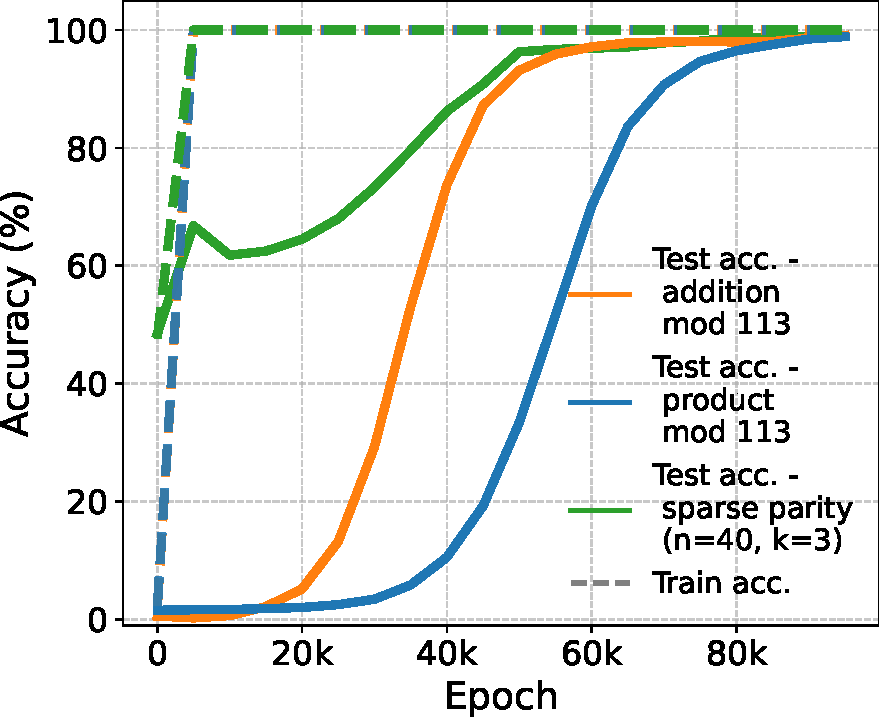
\includegraphics[width=\linewidth]{grokking_iclr_arxiv/figures/stablemax_grokking.pdf}
    %\caption{}
    \label{fig:stablemax_grokking}
\end{subfigure}
\hfill
\begin{subfigure}[t]{.32\textwidth}
    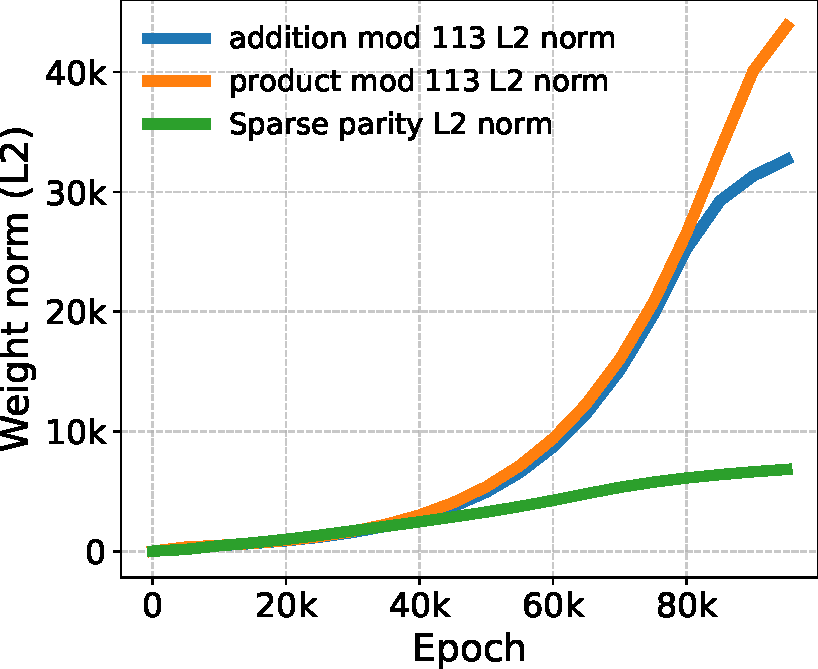
\includegraphics[width=\linewidth]{grokking_iclr_arxiv/figures/weight_norms.pdf}
    %\caption{}
    \label{fig:weight_norms}
\end{subfigure}
\hfill
\begin{subfigure}[t]{.32\textwidth}
    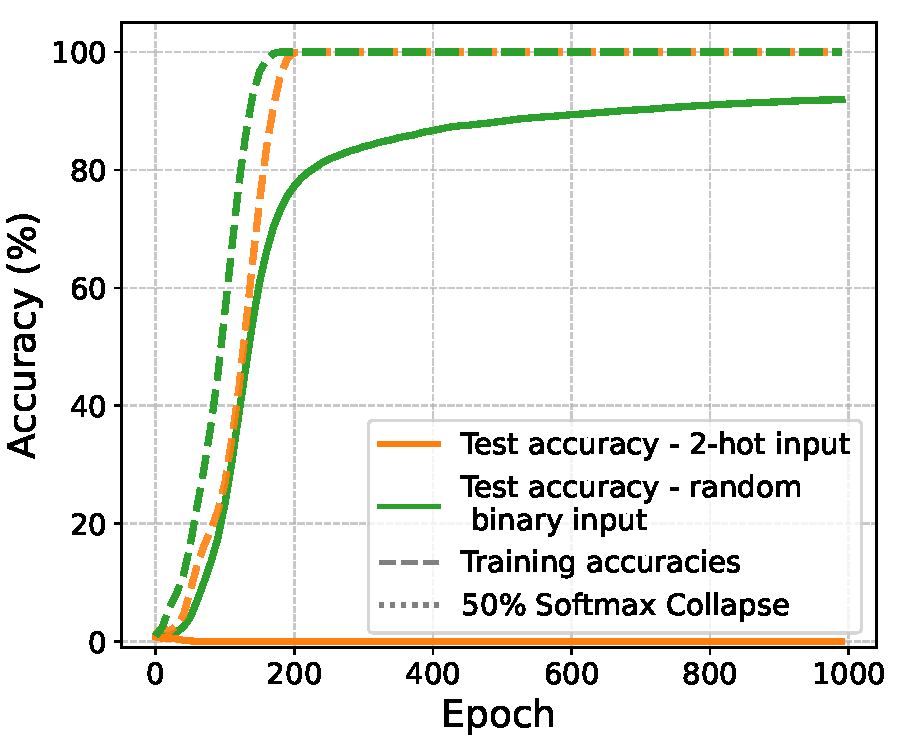
\includegraphics[width=\linewidth]{grokking_iclr_arxiv/figures/input_representations.pdf}
    %\caption{}
\end{subfigure}%
\vspace{-5mm}
    \caption{(\textbf{left}) Grokking with StCE loss and no regularization on three common grokking datasets using an MLP with 2 hidden layers of width 200. We use  40\% of all pairs modulo 113 which is the same setting as \cref{fig:grokking_stops_40} where regular SCE gets stuck at random level performance (random level is 50\% for sparse parity). (\textbf{middle}) Evolution of model weight norms during training for the same models and tasks. This shows that grokking induced without weight decay does not follow the commonly observed trend of rapidly decreasing weight norm during generalization. (\textbf{right}) Changing input representations turns modular addition into regular machine learning tasks with train and test accuracy increasing in tandem, see \cref{sec:nlm}.\vspace{-5mm}}
    \label{fig:input_representations}
\end{figure}

To show that StCE indeed addresses the problems posed by SC, we repeat our experiments in~\cref{sec:evidence-of-sc} by replacing \softmax with $\stablemax$. Our results, presented in \cref{fig:input_representations}, indeed show that $\stablemax$ leads to grokking in commonly studied settings \textit{without} regularization. Notably, this happens while the norm of the weights increases substantially (\cref{fig:input_representations}, middle). This suggests that while weight decay may lead to both grokking and a decreasing weight norm, the decreasing weight norm is not necessary for grokking. Overall, these results i) provide additional evidence for the importance of SC in preventing grokking, ii) suggest a novel activation function to address this problem, and iii) show that regularization or weight norm modification is not \textit{necessary} for grokking.

\begin{comment}
\begin{figure}
\centering
\begin{subfigure}[t]{.65\textwidth}
    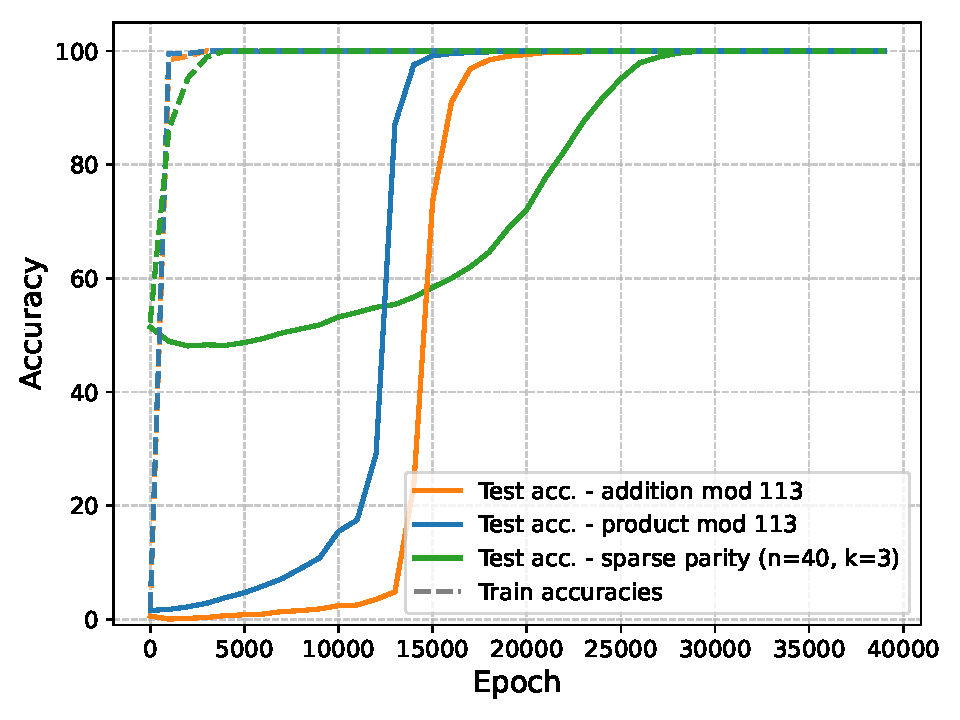
\includegraphics[width=\linewidth]{grokking_iclr/figures/softermax_grokking.pdf}
\end{subfigure}%
\begin{subfigure}[t]{.35\textwidth}
    \raisebox{55pt}[0pt][0pt]{%
    \includegraphics[width=\linewidth]{grokking_iclr/figures/soft_exponential.pdf}}
    
\end{subfigure}%

\caption{Gokking with stable-cross-entropy loss and no regularization on three common grokking datasets using an MLP with 2 hidden layers of width 200. Regular CE  Loss with no regularization gets stuck at random level performance (which is 50\% for sparse parity) in these settings. 40\% of all pairs modulo 113 are used for training on the modular arithmetic tasks.}
\label{fig:stable_max}
\end{figure}
\end{comment}
